\documentclass[tikz,border=5pt]{standalone}
\usepackage[T1]{fontenc}
\usepackage{lmodern,amsmath,amssymb}
\usetikzlibrary{arrows.meta,calc,positioning,fit,backgrounds,shapes.geometric,matrix,decorations.pathreplacing,patterns}
\definecolor{ink}{gray}{0.08}
\definecolor{wash}{gray}{0.965}
\definecolor{soft}{gray}{0.45}
\tikzset{box/.style={draw=ink,line width=.65pt,fill=white,align=center,inner sep=4pt,outer sep=0pt,font=\small},flow/.style={draw=ink,line width=.65pt,-{Latex[length=1.8mm,width=1.3mm]},rounded corners=2pt},annotation/.style={font=\scriptsize,text=soft,align=center},groupbox/.style={draw=soft,dashed,line width=.45pt,fill=wash}}
\begin{document}
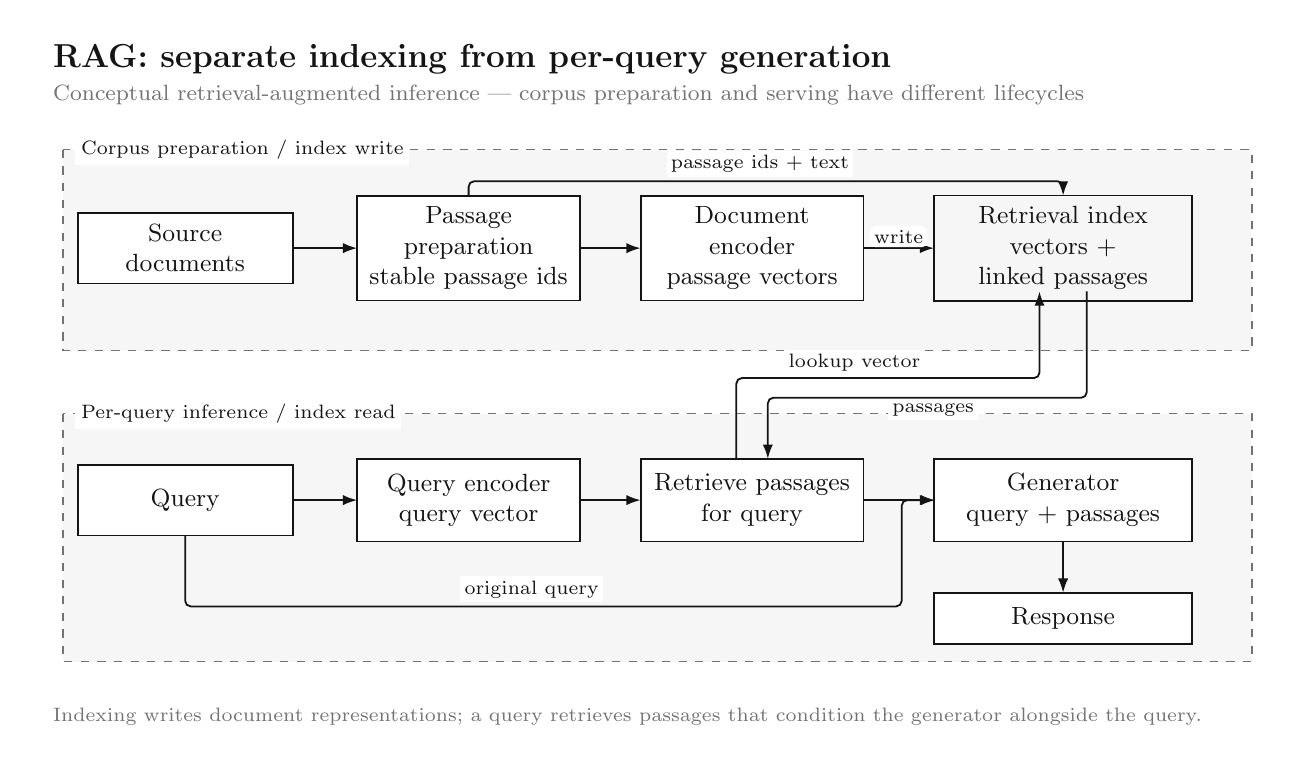
\begin{tikzpicture}[x=1cm,y=-1cm,font=\rmfamily,text=ink]

\path[use as bounding box] (0,0) rectangle (16,9);
\node[anchor=west,font=\large\bfseries] at (.2,.4) {RAG: separate indexing from per-query generation};
\node[anchor=west,font=\footnotesize,text=soft] at (.2,.85) {Conceptual retrieval-augmented inference | corpus preparation and serving have different lifecycles};
\begin{pgfonlayer}{background}
\draw[groupbox] (0.45,1.55) rectangle (15.549999999999999,4.1);
\node[anchor=west,font=\scriptsize,fill=white,inner sep=2pt] at (0.6,1.55) {Corpus preparation / index write};
\draw[groupbox] (0.45,4.9) rectangle (15.549999999999999,8.05);
\node[anchor=west,font=\scriptsize,fill=white,inner sep=2pt] at (0.6,4.9) {Per-query inference / index read};
\end{pgfonlayer}
\node[box,minimum width=2.7cm,minimum height=0.9cm,text width=2.45cm] (docs) at (2.0,2.8) {Source\\documents};
\node[box,minimum width=2.8cm,minimum height=1.05cm,text width=2.55cm] (chunk) at (5.6,2.8) {Passage preparation\\stable passage ids};
\node[box,minimum width=2.8cm,minimum height=1.05cm,text width=2.55cm] (denc) at (9.2,2.8) {Document encoder\\passage vectors};
\node[box,fill=wash,minimum width=3.25cm,minimum height=1.1cm,text width=3.0cm] (index) at (13.15,2.8) {Retrieval index\\vectors + linked passages};
\node[box,minimum width=2.7cm,minimum height=0.9cm,text width=2.45cm] (query) at (2.0,6.0) {Query};
\node[box,minimum width=2.8cm,minimum height=1.05cm,text width=2.55cm] (qenc) at (5.6,6.0) {Query encoder\\query vector};
\node[box,minimum width=2.8cm,minimum height=1.05cm,text width=2.55cm] (retrieve) at (9.2,6.0) {Retrieve passages\\for query};
\node[box,minimum width=3.25cm,minimum height=1.05cm,text width=3.0cm] (generate) at (13.15,6.0) {Generator\\query + passages};
\node[box,minimum width=3.25cm,minimum height=0.65cm,text width=3.0cm] (answer) at (13.15,7.5) {Response};
\begin{pgfonlayer}{background}
\draw[flow] (docs.east) -- (chunk.west);
\draw[flow] (chunk.east) -- (denc.west);
\draw[flow] (denc.east) -- (index.west) node[midway,above,fill=white,inner sep=1.5pt,font=\scriptsize] {write};
\draw[flow] (query.east) -- (qenc.west);
\draw[flow] (qenc.east) -- (retrieve.west);
\draw[flow] (retrieve.east) -- (generate.west);
\draw[flow] (generate.south) -- (answer.north);
\end{pgfonlayer}
\draw[flow] (chunk.north) -- (5.6,1.95) -- (13.15,1.95) -- (index.north);
\node[font=\scriptsize,fill=white,inner sep=1.5pt,anchor=south] at (9.3,1.9) {passage ids + text};
\draw[flow] (9.0,5.475) -- (9.0,4.45) -- (12.85,4.45) -- (12.85,3.35);
\node[font=\scriptsize,fill=white,inner sep=1.5pt,anchor=south] at (10.5,4.42) {lookup vector};
\draw[flow] (13.45,3.35) -- (13.45,4.7) -- (9.4,4.7) -- (9.4,5.475);
\node[font=\scriptsize,fill=white,inner sep=1.5pt,anchor=north] at (11.5,4.72) {passages};
\draw[flow] (2.0,6.45) -- (2.0,7.35) -- (11.1,7.35) -- (11.1,6.0) -- (11.525,6.0);
\node[font=\scriptsize,fill=white,inner sep=1.5pt,anchor=south] at (6.4,7.3) {original query};
\node[anchor=west,align=left,font=\scriptsize,text=soft,text width=15.6cm] at (.2,8.75) {Indexing writes document representations; a query retrieves passages that condition the generator alongside the query.};
\end{tikzpicture}
\end{document}
